\PassOptionsToPackage{table}{xcolor}
\documentclass[nobib,nofonts]{tufte-handout}

%\geometry{showframe} % display margins for debugging page layout

%%% MF additions
% \usepackage[table]{xcolor}
\usepackage[nographicx, nohyperref, nosubcaption, nogb4e, nobiblatex]{../99-auxiliary-files/00-mypackages}
\usepackage{../99-auxiliary-files/00-mycommands}
\usepackage{../99-auxiliary-files/00-myenvironments}

\usepackage{titlesec}
\usepackage{etoolbox}
\usepackage{tikz-qtree}
\usepackage{subcaption}

\usepackage{pgfplots}
% externalize PGF plots
% \usepgfplotslibrary{external}
% \tikzexternalize

% \titleformat{\section}
% {\large\bfshape}{\thesection}{1em}{}

\setcounter{secnumdepth}{5}
\renewcommand\thesection{\arabic{section}}

% this length controls tha hanging indent for titles
% change the value according to your needs
\newlength\titleindent
\setlength\titleindent{0.7cm}

\pretocmd{\paragraph}{\stepcounter{subsection}}{}{}
\pretocmd{\subparagraph}{\stepcounter{subsubsection}}{}{}

\titleformat{\chapter}[block]
  {\normalfont\huge\bfseries}{}{0pt}{\hspace*{-\titleindent}}

\titleformat{\section}
  {\normalfont\Large\itshape}{\llap{\parbox{\titleindent}{\thesection\hfill}}}{0em}{}

\titleformat{\subsection}
  {\normalfont\itshape}{\llap{\parbox{\titleindent}{\thesubsection\hfill}}}{0em}{}

\titleformat{\subsubsection}
  {\normalfont\normalsize\itshape}{\llap{\parbox{\titleindent}{\thesubsubsection}}}{0em}{}

\titleformat{\paragraph}[runin]
  {\normalfont\normalsize\itshape}{}{-0.7cm}{}[\xspace \ \ \ \ ]

\titleformat{\subparagraph}[runin]
  {\normalfont\normalsize}{\llap{\parbox{\titleindent}{\thesubsubsection\hfill}}}{0em}{}

\titlespacing*{\chapter}{0pt}{0pt}{20pt}
\titlespacing*{\subsubsection}{0pt}{3.25ex plus 1ex minus .2ex}{1.5ex plus .2ex}
\titlespacing*{\paragraph}{0pt}{3.25ex plus 1ex minus .2ex}{0em}
\titlespacing*{\subparagraph}{0pt}{3.25ex plus 1ex minus .2ex}{0em}

\DefineNamedColor{named}{mygray2}{cmyk}{0.55,0.25,0.25,0.25}
\newcommand{\mygray}[1]{\textcolor{mygray2}{#1}}

%%% Tufte style
\usepackage{graphicx} % allow embedded images
  \setkeys{Gin}{width=\linewidth,totalheight=\textheight,keepaspectratio}
  \graphicspath{{graphics/}} % set of paths to search for images

\usepackage{fancyvrb} % extended verbatim environments
  \fvset{fontsize=\normalsize}% default font size for fancy-verbatim environments

% Standardize command font styles and environments
\newcommand{\doccmd}[1]{\texttt{\textbackslash#1}}% command name -- adds backslash automatically
\newcommand{\docopt}[1]{\ensuremath{\langle}\textrm{\textit{#1}}\ensuremath{\rangle}}% optional command argument
\newcommand{\docarg}[1]{\textrm{\textit{#1}}}% (required) command argument
\newcommand{\docenv}[1]{\textsf{#1}}% environment name
\newcommand{\docpkg}[1]{\texttt{#1}}% package name
\newcommand{\doccls}[1]{\texttt{#1}}% document class name
\newcommand{\docclsopt}[1]{\texttt{#1}}% document class option name
\newenvironment{docspec}{\begin{quote}\noindent}{\end{quote}}% command specification environment

\newcommand{\proplog}{\acro{PropLog}}
\newcommand{\EFSQ}{\ensuremath{\mathit{EFSQ}}\xspace}

%%%%%%%%%%%%%%%%%%%%%%%%%%%%%%%%%%%%%%%%%%%%%%%%%%

% \usepackage[sc,osf]{mathpazo}
% \linespread{1.05}


\title{Probability theory basics}

\author[M.~Franke]{Michael Franke}

\date{} % without \date command, current date is supplied

\usepackage{epsdice} % for dice

\newcommand{\mult}{\ensuremath{\cdot}}

\begin{document}

\maketitle

\begin{abstract}
\noindent
Basics of probability theory:
axiomatic definition,
interpretation,
joint distributions,
marginalization,
conditional probability,
Bayes rule,
stochastic independence.
Random variables \& expected values.
\end{abstract}

\section{Probability}

\subsection{Relative degrees of credence}

What is the weather going to be like tomorrow: sunny, misty or rainy?\sidenote{
  Let's assume that there are only these three options and that these are mutually exclusive.
}
We do not know, but we may have different beliefs.
Our beliefs might or might not agree in as much as that all three states of the weather are possible, i.e., could actually happen tomorrow.
But even if they do, our beliefs might differ (drammaticallly) regarding the question of how likely each possibility is.

Probabilities are one way of formally representing such beliefs.
Probability distributions assign numbers to possible states of affairs (think: sets of possible worlds).
What matters most about these numbers are the \emph{relative degrees of credence} they express.
Concretely, the information we really care about is that ``sunny'' is deemed to be twice as likely as ``rainy.''
Take an example.

Jones, the optimist, does not know what the weather will bring, but believes that it is most likely to be sunny.
In fact, Jones believes ---for whatever reason--- that it is three times as likely to be sunny than that it is going to be misty.
Jones also believes that being misty and being rainy is equallly likely.
This information about Jones' \emph{relative degrees of credence} alone, is enough to know that, according to Jones, the probability of the three weather conditions are identical to the probability of outcome when turing the wheel of fortune on the left-hand side in Figure~\ref{fig:belief-wheels}.
The area covered by the option ``sunny'' in Jones' wheel of fortune is exactly 60\%, while that of both ``misty'' and ``rainy'' is exactly 20\% each.

Smith is more pessimistic.
Smith's believes that ``misty'' is twice as likely as ``sunny'' and that ``rainy'' is seven times more likely than ``sunny.''
Smith's wheel of fortune is shown on the right-hand side in Figure~\ref{fig:belief-wheels}.

\begin{figure}
  \centering
  \begin{minipage}{0.45\linewidth}
    \centering
    \textbf{Jones}
    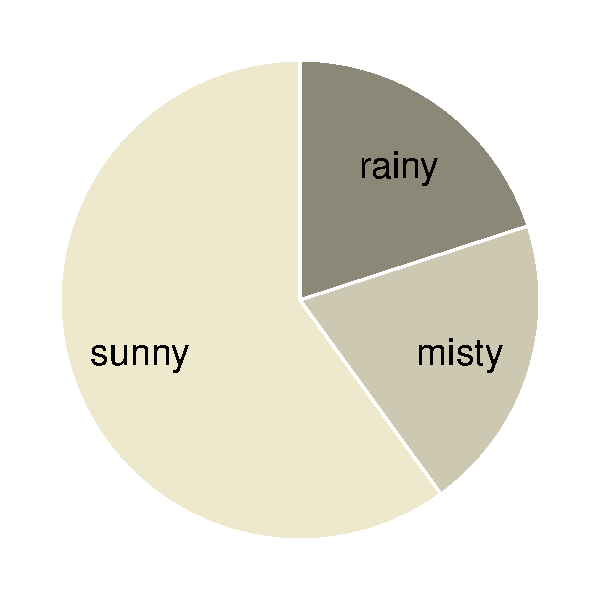
\includegraphics[width=0.9\textwidth]{00-pics/pie-chart-beliefs-Jones.pdf}
  \end{minipage}
  \hfill
  \begin{minipage}{0.45\linewidth}
    \centering
    \textbf{Smith}
    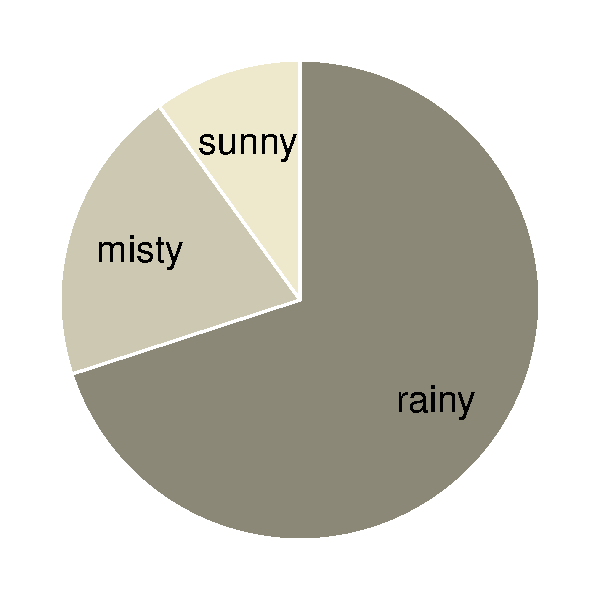
\includegraphics[width=0.9\textwidth]{00-pics/pie-chart-beliefs-Smith.pdf}
  \end{minipage}
  \caption{Two beliefs about the weather, represented as wheels of fortune.}
  \label{fig:belief-wheels}
\end{figure}


Smith, the pessimist, believes that it is surely not going to be sunny.
Probability theory offers a formal representation of uncertainty.

\begin{center}
  \begin{tabular}{lccc}
                    & sunny & cloudy & rainy \\ \midrule
    Jones' beliefs  & 0.6   & 0.2    & 0.2   \\
    Smith's beliefs & 0.1   & 0.2    & 0.7   \\
  \end{tabular}
\end{center}



\subsection{Outcomes, events, observations}

We are interested in the space $\Omega$ of all \markdef{elementary outcomes} $\omega_1,
\omega_2, \dots$ of a process or event whose execution is (partially) random or
unknown. Elementary outcomes are mutually exclusive. The set $\Omega$ exhausts all
possibilities.\sidenote{For simplicity of exposure, we gloss over subtleties arising when
  dealing with infinite sets $\Omega$. We make up for this when we define probability
  \emph{density} functions for continuous random variables, which is all the uncountable
  infinity that we will usually be concerned with in applied statistics.}

\begin{example}
  The set of elementary outcomes of a single coin flip is $\Omega_{\text{coin flip}} =
  \set{\text{heads}, \text{tails}}$. The elementary outcomes of tossing a six-sided die is
  $\Omega_{\text{standard die}} = \set{\epsdice{1}, \epsdice{2}, \epsdice{3}, \epsdice{4},
    \epsdice{5}, \epsdice{6}}$.\sidenote{Think of $\Omega$ as a partition of the space of all possible ways in
  which the world could be, where we lump together into one partition cell all ways in which
  the world could be that are equivalent regarding those aspects of reality that we are
  interested in. We do not care whether the coin lands in the mud or in the sand. It only
  matters whether it came up heads or tails. Each elementary event can be realized in myriad
  ways. $\Omega$ is our, the modellers', first crude simplification of nature, abstracting away aspects we
  currently do not care about.}
\end{example}

An \markdef{event} $A$ is a subset of $\Omega$. Think of an event as a (possibly partial)
observation. We might observe, for instance, not the full outcome of tossing a die, but only
that there is a dot in the middle. This would correspond to the event
$A = \set{\epsdice{1}, \epsdice{3}, \epsdice{5}} \subseteq \Omega_{\text{standard die}}$,
i.e., observing an odd numbered outcome. The trivial observation $A = \Omega$ and the
impossible observation $A = \emptyset$ are counted as events, too. The latter is included for
technical reasons.


For any two events $A, B \subseteq \Omega$, standard set operations correspond to logical
connections in the usual way. For example, the conjunction $A \cap B$ is the observation of
both $A$ and $B$; the disjunction $A \cup B$ is the observation that it is either $A$ or $B$;
the negation of $A$, $\overline{A} = \set{\omega \in \Omega \mid \omega \not \in A}$, is the
observation that it is not $A$.

\subsection{Probability distribution}

A \markdef{probability distribution} $P$ over $\Omega$ is a function
$P \mycolon \pow{\Omega} \rightarrow \mathds{R}$ that assigns to all events
$A \subseteq \Omega$ a real number (from the unit interval, see A1), such that the following
(so-called Kolmogorov axioms) are satisfied:
\begin{enumerate}[{A}1.]
\item $0 \le P(A) \le 1$
\item $P(\Omega) = 1$
\item $P(A_1 \cup A_2 \cup A_3 \cup \dots) = P(A_1) + P(A_2) + P(A_3) + \dots $ whenever $A_1, A_2,
  A_3, \dots$ are mutually exclusive\sidenote{A3 is the axiom of \emph{countable
      additivity}. Finite additivity may be enough for finite or countable sets $\Omega$, but
    infinite additivity is necessary for full generality in the uncountable case.}
\end{enumerate}
Occasionally we encounter notation $P \in \Delta(\Omega)$ to express that $P$ is a probability
distribution over $\Omega$.\sidenote{E.g., in physics, theoretical economics or game
  theory. Less so in psychology or statistics.} If $\omega \in \Omega$ is an elementary event,
we often write $P(\omega)$ as a shorthand for $P(\set{\omega})$. In fact, if $\Omega$ is
finite, it suffices to assign probabilities to elementary outcomes.

A number of rules follow immediately from of this definition:\sidenote[][1em]{Prove this!}
\begin{enumerate}[{C}1.]
\item $P(\emptyset) = 0$
\item $P(\overline{A}) = 1 - P(A)$
\item $P(A \cup B) = P(A) + P(B) - P(A \cap B)$ for any $A, B \subseteq \Omega$
\end{enumerate}


\subsection{Interpretations of probability}

It is reasonably safe, at least preliminarily, to think of probability, as defined above, as a
handy mathematical primitive which is useful for certain applications. There are at least three
ways of thinking about where this primitive probability might come from, roughly paraphrasable
like so:
\begin{enumerate}[1.]
\item \markdef{Frequentist:} Probabilities are generalizations of intuitions/facts about frequencies of events in
  repeated executions of a random event.
\item \markdef{Subjectivist:} Probabilities are subjective beliefs by a rational agent who is
  uncertain about the outcome of a random event.
\item \markdef{Realist:} Probabilities are a property of an intrinsically random world.
\end{enumerate}

\subsection{Urns and frequencies}

Think of an urn as a container which contains a number of $N > 1$ balls. Balls can be of
different color. For example, let us suppose that our urn has $k > 0$ black balls and $N-k$
white balls. (There is at least one black and one white ball.) For a single random draw from
our urn we have: $\Omega_{\text{our urn}} = \set{\text{white}, \text{black}}$. If we imagine an
infinite sequence of single draws from our urn, putting whichever ball we drew back in after
every draw, the limiting proportion with which we draw a black ball is
$\frac{k}{N}$.\sidenote{If in doubt, execute this experiment. By hand or by computer.} This
statement about frequency is what motivates saying that the probability of drawing a black ball
on a single trial is (or should be\sidenote{If probabilities are subjective beliefs, a rational
  agent is, in a sense, normatively required to assign exactly this probability.})
$P(\text{black}) = \frac{k}{N}$.

\section{Structured events \& marginal distributions}

\subsection{Probability table for a flip-\&-draw scenario}

Suppose we have two urns. Both have $N=10$ balls. Urn 1 has $k_1=2$ black and $N-k_1 = 8$ white
balls. Urn 2 has $k_2=4$ black and $N-k_2=6$ white balls. We sometimes draw from urn 1,
sometimes from urn 2. To decide, we flip a fair coin. If it comes up heads, we draw from urn 1;
if it comes up tails, we draw from urn 2.

An elementary outcome of this two-step process of flip-\&-draw is a pair
$\tuple{\text{outcome-flip}, \text{outcome-draw}}$. The set of all possible such outcomes is
$\Omega_{\text{flip-\&-draw}} = \set{\tuple{\text{heads}, \text{black}}, \tuple{\text{heads},
    \text{white}}, \tuple{\text{tails}, \text{black}}, \tuple{\text{tails},
    \text{white}}}$. The probability of event $\tuple{\text{heads}, \text{black}}$ is given by
multiplying the probability of seeing ``heads'' on the first flip, which happens with
probability $0.5$, and then drawing a black ball, which happens with probability $0.2$, so that
$P(\tuple{\text{heads}, \text{black}}) = 0.5 \cdot 0.2 = 0.1$. The probability distribution
over $\Omega_{\text{flip-draw}}$ is consequently as in
Table~\ref{tab:flip-and-draw:probabilities}.\sidenote{If in doubt, start flipping \&
  drawing and count your outcomes.}
%
\begin{table}
  \centering
  \begin{tabular}{lcc}
    & black & white \\ \midrule
    heads & $0.5 \mult 0.2 = 0.1$  & $0.5 \mult 0.8 = 0.4$ \\
    tails & $0.5 \mult 0.4 = 0.2$  & $0.5 \mult 0.6 = 0.3$
  \end{tabular}
  \caption{Probabilities of elementary outcomes (pairs of $\tuple{\text{outcome-flip},
      \text{outcome-draw}}$) in the flip-\&-draw example.}
  \label{tab:flip-and-draw:probabilities}
\end{table}

\subsection{Structured events and joint-probability distributions}

Table~\ref{tab:flip-and-draw:probabilities} is an example of a \markdef{joint
  probability distribution} over a structured event space, which here has two dimensions. Since
our space of outcomes is the Cartesian product of two simpler outcome spaces, namely
$\Omega_{flip-\&-draw} = \Omega_{flip} \times \Omega_{draw}$,\sidenote{With
  $\Omega_{\text{flip}} = \set{\text{heads}, \text{tails}}$ and
  $\Omega_{\text{draw}} = \set{\text{black}, \text{white}}$.} we can use notation
$P(\text{heads}, \text{black})$ as shorthand for $P(\tuple{\text{heads}, \text{black}})$. More
generally, if $\Omega = \Omega_1 \times \dots \Omega_n$, we can think of $P \in \Delta(\Omega)$
as a joint probability distribution over $n$ subspaces.

\subsection{Marginalization}

If $P$ is a joint-probability distribution over event space $\Omega = \Omega_1 \times \dots
\Omega_n$, the \markdef{marginal distribution} over subspace  $\Omega_i$, $1 \le
i \le n$ is the probability distribution that assigns to all $A_i \subseteq \Omega_i$ the probability:\sidenote{This
  notation, using $\sum$, assumes that subspaces are countable. In other cases, a parallel
  definition with integrals can be used.}
\begin{align*}
  P(A_i) = \sum_{A_1 \subseteq \Omega_{1}, \dots , A_{i-1} \subseteq \Omega_{i-1}, A_{i+1} \subseteq \Omega_{i+1}, \dots, A_n \subseteq
    \Omega_n} P(A_1, \dots, A_{i-1}, A_{i}, A_{i+1}, \dots A_n)
\end{align*}
For example, the marginal distribution over coin flips derivable from the joint probability
distribution in Table~\ref{tab:flip-and-draw:probabilities} gives $P(\text{heads}) = P(\text{tails}) =
0.5$, since the sum of each row is exactly $0.5$. The marginal distribution over flips
derivable from Table~\ref{tab:flip-and-draw:probabilities} has $P(\text{black}) = 0.3$ and
$P(\text{black}) = 0.7$.\sidenote{The term ``marginal distribution'' derives from such
  probability tables, where traditionally the sum of each row/column was written in the
  margins.}

\section{Conditional probability}

Fix probability distribution $P \in \Delta(\Omega)$ and events $A,B \subseteq \Omega$. The
conditional probability of $A$ given $B$, written as $P(A \mid B)$, gives the probability of
$A$ on the assumption that $B$ is true.\sidenote{We also verbalize this as ``the conditional
  probability of $A$ conditioned on $B$.''} It is defined like so:
\begin{align*}
  P(A \mid B) = \frac{P(A \cap B)}{P(B)}
\end{align*}
Conditional probabilities are only defined when $P(B) > 0$.\sidenote{Updating with events which have
probability zero entails far more severe adjustments of the underlying belief system than just
ruling out information hitherto considered possible. Formal systems that capture such
\emph{belief revision} are studied in formal epistemology.}


\begin{example}
  If a dice is unbiased, each of its six faces has equal probability to come up after a toss. The
  probability of event $B = \set{\epsdice{1}, \epsdice{3}, \epsdice{5}}$ that the tossed number
  is odd has probability $P(B) = \frac{1}{2}$. The probability of event $A = \set{\epsdice{3}, \epsdice{4},
    \epsdice{5}, \epsdice{6}}$ that the tossed number is bigger than two is $P(A) =
  \frac{2}{3}$. The probability that the tossed number is bigger than two \emph{and} odd is
  $P(A \cap B) = P(\set{\epsdice{3}, \epsdice{5}}) = \frac{1}{3}$. The conditional probability
  of tossing a number that is bigger than two, when we know that the toss is even, is $P(A \mid
  B) = \frac{\nicefrac{1}{3}}{\nicefrac{1}{2}} = \frac{2}{3}$.
\end{example}

Algorithmically, conditional probability first rules out all events in which $B$ is not true
and then simply renormalizes the probabilities assigned to the remaining events in such a way
that the relative probabilities of surviving events remains unchanged. Given this, another way
of interpreting conditional probability is that $P(A \mid B)$ is what a rational agent
\emph{should} believe about $A$ after observing that $B$ is in fact true and nothing more. The
agent rules out, possibly hypothetically, that $B$ is false, but otherwise does not change
opinion about the relative probabilities of anything that is compatible with $B$.

\subsection{Bayes rule}

Looking back at the joint-probability distribution in
Table~\ref{tab:flip-and-draw:probabilities}, the conditional probability
$P(\text{black} \mid \text{heads})$ of drawing a black ball, given that the initial coin flip
showed heads, can be calculated as follows:
\begin{align*}
  P(\text{black} \mid \text{heads}) = \frac{P(\text{black} , \text{heads})}{P(\text{heads})} =
  \frac{0.1}{0.5} = 0.2
\end{align*}
This calculation, however, is quite spurious. We knew that already from the way the
flip-\&-draw scenario was set up. After flipping heads, we draw from urn 1, which has $k=2$ out
of $N=10$ black balls, so clearly: if the flip is heads, then the probability of a black ball
is $0.2$. Indeed, in a step-wise random generation process like the flip-\&-draw scenario, some
conditional probabilities are very clear, and sometimes given by definition. These are,
usually, the conditional probabilities that define how the process unfolds forward in time, so
to speak.

\markdef{Bayes rule} is a way of expressing, in a manner of speaking, conditional probabilities in terms of the
``reversed'' conditional probabilities:
\begin{align*}
  P(B \mid A) = \frac{P(A \mid B) \mult P(B)}{P(A)}
\end{align*}
Bayes rule is straightforward corollary of the definition of conditional probabilities,
according to which $P(A \cap B) = P(A \mid B) \mult P(B)$, so that:
\begin{align*}
  P(B \mid A) = \frac{P(A \cap B)}{P(A)} = \frac{P(A \mid B) \cdot P(B)}{P(A)}
\end{align*}

Bayes rule allows for reasoning backwards from observed causes to likely underlying effects.
When we have a feed-forward model of how unobservable effects probabilistically constrain
observable outcomes, Bayes rule allows us to draw inferences about \emph{latent/unobservable
  variables} based on the observation of their downstream effects.

Consider yet again the flip-\&-draw scenario. But now assume that Jones flipped the coin and
drew a ball. We see that it is black. What is the probability that it was drawn from urn 1,
equivalently, that the coin landed heads? It is not $P(\text{heads}) = 0.5$, the so-called
\emph{prior probability} of the coin landing heads. It is a conditional probability, also
called the \emph{posterior probability},\sidenote{The terms \emph{prior} and \emph{posterior}
  make sense when we think about an agent's belief state before (prior to) and after (posterior
  to) an observation.} namely $P(\text{heads} \mid \text{black})$, but one
that is not as easy and straightforward to write down as the reverse
$P(\text{black} \mid \text{heads})$ of which we said above that it is an almost trivial part of
the set up of the flip-\&-draw scenario. It is here that Bayes rule has its purpose:
\begin{align*}
  P(\text{heads} \mid \text{black}) = \frac{P(\text{black} \mid \text{heads}) \mult P(\text{heads})}{P(\text{black})} =
  \frac{0.2 \mult 0.5}{0.3} = \frac{1}{3}
\end{align*}
This result is quite intuitive. Drawing a black ball from urn 2 (i.e., after seeing tails) is twice
as likely as drawing a black ball from urn 1 (i.e., after seeing heads). Consequently, after
seeing a black ball drawn, with equal probabilities of heads and tails, the probability that
the coin landed tails is also twice as large as that it landed heads.

\section{Random variables}

We have so far define a probability distribution as a function that assigns a probability to
each subset of the space $\Omega$ of elementary outcomes. A special case occurs when we are
interested in a space of numeric outcomes.

A \markdef{random variable} is a function $X \mycolon \Omega \rightarrow \mathds{R}$ that
assigns to each elementary outcome a numerical value.

\begin{example}
  For a single flip of a coin we have $\Omega_{\text{coin flip}} =
  \set{\text{heads}, \text{tails}}$. A usual way of mapping this onto numerical outcomes is to
  define $X_{\text{coin flip}} \mycolon \text{heads} \mapsto 1; \text{tails} \mapsto 0$. Less trivially, consider
  flipping a coin two times. Elementary outcomes should be individuated by the outcome of the
  first flip and the outcome of the second flip, so that we get:
  \begin{align*}
    \Omega_{\text{two flips}} = \set{\tuple{\text{heads}, \text{heads}}, \tuple{\text{heads}, \text{tails}},
    \tuple{\text{tails}, \text{heads}}, \tuple{\text{tails}, \text{tails}}}
  \end{align*}
  Consider the random variable $X_{\text{two flips}}$ that counts the
  total number of heads. Crucially,
  $X_{\text{two flips}}(\tuple{\text{heads}, \text{tails}}) = 1 = X_{\text{two
      flips}}(\tuple{\text{tails}, \text{heads}})$. We assign the same numerical value to
  different elementary outcomes.
\end{example}


\subsection{Notation \& terminology}

Traditionally random variables are represented by capital letters, like $X$. Variables for the
numeric values they take on are written as small letters, like $x$.

We write $P(X = x)$ as a shorthand for the probability
$P(\set{\omega \in \Omega \mid X(\omega) = 2})$ that an event occurs that is mapped onto $x$ by
random variable $X$. For example, if our coin is fair, then $P(X_{\text{two flips}} = x) = 0.5$
for $x=1$ and $0.25$ otherwise. Similarly, we can also write $P(X \le x)$ for the probability
of observing an event that $X$ maps to a number not bigger than $x$.

If the range of $X$ is countable, we say that $X$ is \markdef{discrete}. For ease of
exposition, we may say that if the range of $X$ is an interval of real numbers, $X$ is
called \markdef{continuous}.

\subsection{Cumulative distribution functions, mass and density}

For a discrete random variable $X$, the \markdef{cumulative distribution function} $F_X$
associated with $X$ is defined as:
\begin{align*}
  F_X(x) = P(X \le x) = \sum_{x' \in \set{\text{Rng}(X) \mid x' \le x}} P(X = x)
\end{align*}
The \markdef{probability mass function} $f_x$ associated with $X$ is defined as:
\begin{align*}
  f_X(x) = P(X = x)
\end{align*}

\begin{example}
  Suppose we flip a coin with a bias of $\theta$ $n$ times. What is the probability that we
  will see heads $k$ times? If we map the outcome of heads to 1 and tails to 0, this
  probability is given by the \markdef{Binomial distribution}, as follows:
  \begin{align*}
    \text{Binom}(K = k ; n, \theta) = \binom{n}{k} \,  \theta^{k} \, (1-\theta)^{n-k}
  \end{align*}
  Here $\binom{n}{k} = \frac{n!}{k!(n-k)!}$ is the binomial coefficient. It gives the number
  possibilities of drawing an unordered set with $k$ elements from a set with a total of $n$
  elements. Figure~\ref{fig:BinomialDistribution} gives an example of the Binomial
  distribution, concretely its probability mass function, for two values of the coin's bias,
  $\theta = 0.25$ or $\theta = 0.5$, when flipping the coin $n=24$
  times. Figure~\ref{fig:BinomialDistributionCumulative} gives the corresponding cumulative
  distributions.
  %% add some more explanation

\begin{figure}
  \centering
  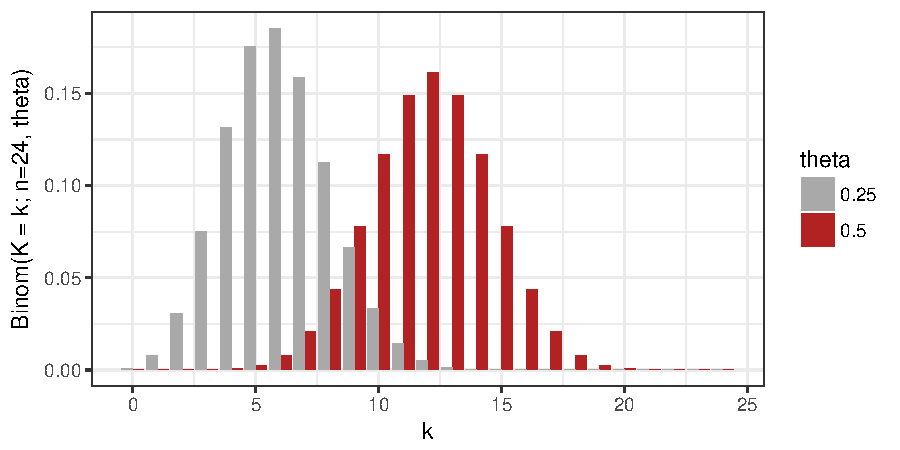
\includegraphics[width=\textwidth]{00-pics/05_00_binomial-distribution.pdf}
  \caption{Examples of the Binomial distribution. The $y$-axis give the probability of seeing
    $k$ heads when flipping a coin $n=24$ times with a bias of either $\theta = 0.25$ or
    $\theta = 0.5$.}
  \label{fig:BinomialDistribution}
\end{figure}

\begin{figure}
  \centering
  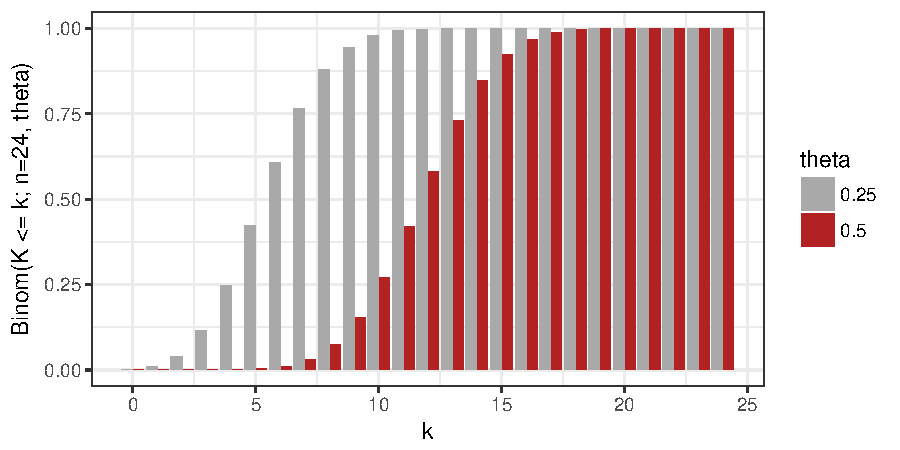
\includegraphics[width=\textwidth]{00-pics/05_00_binomial-distribution-cumulative.pdf}
  \caption{Examples of the cumulative distribution of the Binomial. The $y$-axis gives the
    probability of seeing $k$ or less outcomes of heads when flipping a coin $n=24$ times with
    a bias of either $\theta = 0.25$ or $\theta = 0.5$.}
  \label{fig:BinomialDistributionCumulative}
\end{figure}

\end{example}

For a continuous random variable $X$, the probability $P(X = x)$ will usually be zero: it is
virtually impossible that we will see precisely the value $x$ realized in a random event that
can realize uncountably many numerical values of $X$. However, $P(X \le x)$ does take workable
values and so we define the \markdef{cumulative distribution function} $F_X$
associated with $X$ as:
\begin{align*}
  F_X(x) = P(X \le x)
\end{align*}
Instead of a probability \emph{mass} function, we derive a \markdef{probability density
  function} from the cumulative function as:
\begin{align*}
  f_X(x) = F'(x)
\end{align*}
A probability density function can take values greater than one, unlike a probability mass
function.

\begin{example}
  The \markdef{Gaussian or Normal distribution} characterizes many natural distributions of
  measurements which are symmetrically spread around a central tendency. It is defined as:
  \begin{align*}
    \mathcal{N}(X = x ; \mu, \sigma) = \frac{1}{\sqrt{2 \sigma^2 \pi}} \exp \left ( -
      \frac{(x-\mu)^2}{2 \sigma^2} \right)
  \end{align*}
  where parameter $\mu$ is the \emph{mean}, the central tendency, and parameter $\sigma$ is the
  \emph{standard deviation}. Figure~\ref{fig:NormalDistribution} gives examples of the
  probability density function of two normal
  distributions. Figure~\ref{fig:NormalDistributionCumulative} gives the corresponding
  cumulative distribution functions.

\begin{figure}
  \centering
  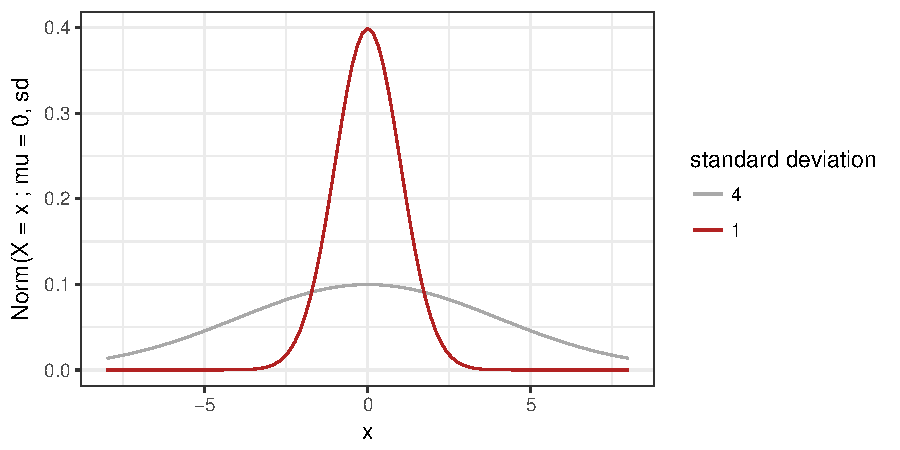
\includegraphics[width=\textwidth]{00-pics/05_01_normal-distribution.pdf}
  \caption{Examples of the Normal distribution. In both cases $\mu = 0$, once with $\sigma = 1$
    and once with $\sigma = 4$.}
  \label{fig:NormalDistribution}
\end{figure}

\begin{figure}
  \centering
  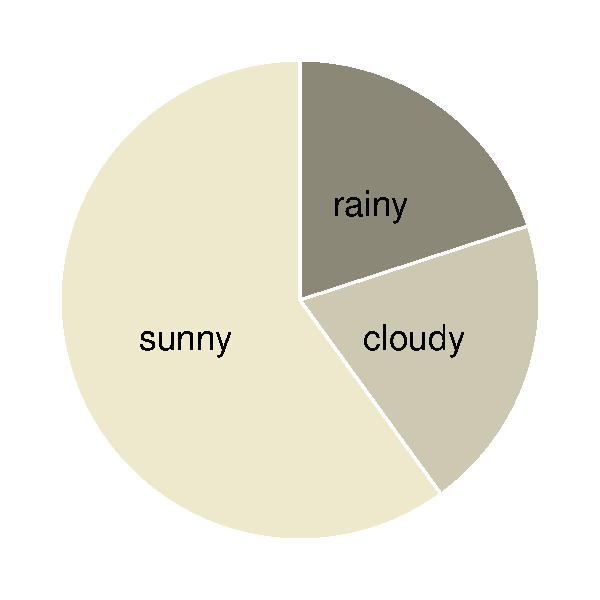
\includegraphics[width=\textwidth]{00-pics/05_01_normal-distribution-cumulative.pdf}
  \caption{Examples of the cumulative normal distribution corresponding to the previous probability
    density functions.}
  \label{fig:NormalDistributionCumulative}
\end{figure}

\end{example}

\subsection{Expected value \& variance}

The \markdef{expected value} of a random variable $X$ is a measure of central tendency. It
tells us, like the name suggests, which average value of $X$ we can expect when repeatedly
sampling from $X$. If $X$ is continuous, the expected value is:\sidenote{The expected value is
  also frequently called the \emph{mean}.}
\begin{align*}
  \mathds{E}_X = \sum_{x} x \mult f_X(x)
\end{align*}
If $X$ is continuous, it is:
\begin{align*}
  \mathds{E}_X = \int x \mult f_X(x) \ \text{d}x
\end{align*}

The \markdef{variance} of a random variable $X$ is a measure of how much likely values of $X$
are spread or clustered around the expected value. If $X$ is discrete, the variance is:
\begin{align*}
  \text{Var}(X) = \sum_x (\mathds{E}_X - x)^2 \mult f_X(x)
\end{align*}
If $X$ is continuous, it is:
\begin{align*}
  \text{Var}(X) = \int (\mathds{E}_X - x)^2 \mult f_X(x) \ \text{d}x
\end{align*}

\begin{example}
  If we flip a coin with bias $\theta = 0.25$ a total of $n=24$, we expect on average to see
  $n \mult \theta = 24 \mult 0.25 = 6$ outcomes showing heads.\sidenote{This is not immediately
    obvious from our definition, but it is intuitive and you can derive it.} The variance is
  $n \mult \theta \mult (1-\theta) = 24 \mult 0.25 \mult 0.75 = \frac{24 \mult 3}{16} =
  \frac{18}{4} = 4.5$.

  The expected value of a normal distribution is just its mean $\mu$ and its variance is
  $\sigma^2$.
\end{example}

% \printbibliography

\end{document}
